%
% This is the LaTeX template file for preparing lecture notes for 
% courses taught by Neil Calkin.  When preparing 
% LaTeX notes for this class, please use this template.
%
% The body contains examples: study them, run 
%
% pdflatex <yourfilename.tex>
%
% and see how they work.   View the output file with acrobat,
% or print it out to compare input and result.
%
%
%
%
%


\documentclass{article}
\usepackage{epsfig,amsmath,amssymb}
\usepackage{graphicx}
\usepackage[myheadings]{fullpage}

% Erin's additions
\usepackage{color} 
\usepackage{tikz}
\usetikzlibrary{decorations.pathmorphing}
\usetikzlibrary{decorations.fractals}

%
% The following commands set up the lecnum (lecture number)
% counter and make various numbering schemes work relative
% to the lecture number.
%
\newcounter{lecnum}
\renewcommand{\thepage}{\thelecnum-\arabic{page}}
\renewcommand{\thesection}{\thelecnum.\arabic{section}}
\renewcommand{\theequation}{\thelecnum.\arabic{equation}}
\renewcommand{\thefigure}{\thelecnum.\arabic{figure}}
\renewcommand{\thetable}{\thelecnum.\arabic{table}}

%
% The following macro is used to generate the header.
%
\newcommand{\lecture}[4]{
   \pagestyle{myheadings}
   \thispagestyle{plain}
   \newpage
   \setcounter{lecnum}{#1}
   \setcounter{page}{1}
   \noindent
   \begin{center}
   \framebox{
      \vbox{\vspace{2mm}
    \hbox to 6.28in { {\bf Combinatorial Analysis
                        \hfill Fall 2010} }
       \vspace{4mm}
       \hbox to 6.28in { {\Large \hfill Lecture #1: #2  \hfill} }
       \vspace{2mm}
       \hbox to 6.28in { {\it Lecturer: #3 \hfill Scribe: #4} }
      \vspace{2mm}}
   }
   \end{center}
   \markboth{Lecture #1: #2}{Lecture #1: #2}
   {\bf Disclaimer}: {\it These notes are intended for students in the class
listed above: they are not guaranteed to be complete or even necessarily
correct.  They may only be redistributed with permission, which you may
expect will be liberally granted.  Ask first, please.} \vspace*{4mm}
}

%
% Convention for citations is authors' initials followed by the year.
% For example, to cite a paper by Leighton and Maggs you would type
% \cite{LM89}, and to cite a paper by Strassen you would type \cite{S69}.
% (To avoid bibliography problems, for now we redefine the \cite command.)
% Also commands that create a suitable format for the reference list.
\renewcommand{\cite}[1]{[#1]}
\def\beginrefs{\begin{list}%
        {[\arabic{equation}]}{\usecounter{equation}
         \setlength{\leftmargin}{2.0truecm}\setlength{\labelsep}{0.4truecm}%
         \setlength{\labelwidth}{1.6truecm}}}
\def\endrefs{\end{list}}
\def\bibentry#1{\item[\hbox{[#1]}]}

%Use this command for a figure; it puts a figure in wherever you want it.
%usage: \fig{NUMBER}{SPACE-IN-INCHES}{CAPTION}
\newcommand{\fig}[3]{
      \vspace{#2}
      \begin{center}
      Figure \thelecnum.#1:~#3
      \end{center}
  }
% Use these for theorems, lemmas, proofs, etc.
\newtheorem{theorem}{Theorem}[lecnum]
\newtheorem{lemma}[theorem]{Lemma}
\newtheorem{proposition}[theorem]{Proposition}
\newtheorem{claim}[theorem]{Claim}
\newtheorem{corollary}[theorem]{Corollary}
\newtheorem{definition}[theorem]{Definition}
\newenvironment{proof}{{\bf Proof:}}{\hfill\rule{2mm}{2mm}}


\def\Z{\hbox{$\mathbb Z$}}
\def\Q{\hbox{$\mathbb Q$}}
\def\R{\hbox{$\mathbb R$}}
\def\N{\hbox{$\mathbb N$}}
\def\C{\hbox{$\mathbb C$}}



% **** IF YOU WANT TO DEFINE ADDITIONAL MACROS FOR YOURSELF, PUT THEM HERE:
\allowdisplaybreaks

\def\e{\hbox{$\mathcal E$}}
\def\o{\hbox{$\mathcal O$}}

\def\bea{\begin{eqnarray*}}
\def\eea{\end{eqnarray*}}

\def\A{\hbox{$\mathcal A$}}
\def\B{\hbox{$\mathcal B$}}



\begin{document}
%FILL IN THE RIGHT INFO.
%\lecture{**LECTURE-NUMBER**}{**DATE**}{**LECTURER**}{**SCRIBE**}
\lecture{13}{September 15}{Neil Calkin}{Erin Doolittle and Dominic Morgan}


\begin{flushleft}
\section{Integer Partitions}
Computing p(n) via $np_n = \sum\limits_{0 \leq k \leq n-1}{p_k \sigma (n-k)}$ requires $\theta (n)$ multiplications for $p_n$ and $\theta (n)$ additions, one division, and hence $\theta (n^2)$ additions and multiplications and $\theta(n)$ divisions to compute $p_0$, $p_1$, $\ldots$, $p_n$.\\
\vspace{4mm}

\underline{Aside}: $f(n) = \theta (g(n))$ means $\exists c_1$,$c_2 > 0$ s.t. $c_1 g(n) \leq | f(n)| \leq c_2 g(n)$. Here g(n) will be a positive function.\\
\vspace{4mm}

Computing $\sigma(1)$, $\sigma(2)$, $\ldots$, $\sigma(n)$ can be done with $< n\left(1+\frac{1}{2}+\frac{1}{3}+\frac{1}{4}+\ldots+\frac{1}{n}\right)$ operations:\\
\vspace{3mm}
for $j$ from 1 to $n \hspace{4mm} \sigma(j) = 1$ end\\ %Psuedocode
for $j$ from 2 to $n$\\
\hspace{4mm} for $k$ from 1 to $\lfloor \frac{n}{j} \rfloor$\\
\hspace{9mm} $\sigma(jk) = \sigma(jk)+j$\\
\hspace{4mm} end\\
end\\

\begin{center}
\begin{tabular}{c c c c c c c c c}
1 & 2 & 3 & 4 & 5 & 6 & 7 & 8 & 9\\
1 & 1 & 1 & 1 & 1 & 1 & 1 & 1 & 1 \\
   & 3 &    & 3 &    & 3 &    & 3 & 1 \\
   &    & 4 &    &    & 6 &    &    & 4 \\
   &    &    & 7 &    &    &    & 7 & \\
   &    &    &    & 6 &    &    &    & \\
   &    &    &    &    & 12 &    &    & \\
   &    &    &    &    &    & 8 &    & \\
   &    &    &    &    &    &    & 15 & \\
   &    &    &    &    &    &    &    & 13\\
\end{tabular}
\end{center}

$n+\lfloor \frac{n}{2}\rfloor+\lfloor \frac{n}{3} \rfloor + \ldots+\lfloor \frac{n}{2} \rfloor < n \left( \frac{1}{1} + \frac{1}{2} + \ldots + \frac{1}{n} \right) = n H_n$\\
\vspace{2mm}
$H_n =\log{n} + \gamma + O\left( \frac{1}{n} \right)$\\
\vspace{2mm}
So number of operations is $< n$ log $n + O(n)$ (incrementing by 1).\\
General: Suppose $f_n$ is a non-negative sequence and that $f(x) = \sum\limits_{n \geq 0}{f_n x^n}$ has radius of convergence R. Then, for any $x \in (0,R)$, $f_n x^n \leq f(x)$.\\
\vspace{2mm}
Hence $f_n \leq \inf\limits_{x \in (0,R)} \frac{f(x)}{x^n}$.\\
\vspace{2mm}
Hence, if we solve $ \frac{f'(x)}{x^n} -  \frac{nf(x)}{x^n} = 0$, that is, $ x =  \frac{nf(x)}{f'(x)}$ say for $x^*$, $f_n \leq  \frac{f(x^*)}{(x^*)^n}$.\\
\newpage

\underline{Example}: $f_n = \frac{1}{n!}$, $f(x)=e^x \Rightarrow f'(x)=e^x$, so $x^* = n$ and $\frac{1}{n!} \leq \frac{e^9}{n}$ or $n! \geq \left(\frac{n}{e}\right)^n$.   \\
\vspace{2mm}
Truth: $n!\sim \left(\frac{n}{e}\right)^n\sqrt{2 \pi n}$ that is $\frac{n!}{\left(\frac{n}{e}\right)^n \sqrt{2 \pi n}} \rightarrow 1$ as $n \rightarrow \infty$.\\
\vspace{2mm}
Fairly typical behavior: If $f_n$ grows nicely, "smoothly", then we obtain $f_n < \frac{f(x^*)}{(x^*)^n}$ and the "truth" is $f_n \sim \frac{c}{n^{\alpha}} \frac{f(x^*)}{(x^*)^n}$\\
\vspace{2mm}
$p_n = [x^n] \prod\limits_{k=1}^{\infty}{(1-x^k)^{-1}} =  [x^n] \prod\limits_{k=1}^{n}{(1-x^k)^{-1}}$ \\
\vspace{2mm}
So we can obtain an upperbound for $p_n$ by $p_n \leq \frac{\prod\limits_{k=1}^{n}{(1-x^k)^{-1}}}{x^n}$.\\

\vspace{3mm}
\textbf{
{\color{red}Exercise: How good a bound can you use this to give? Hint: $p_n \leq \sum\limits_{k=1}^{n}{-\log{(1-x^k)}-n\log{x}}$}}\\
\end{flushleft}

\section{Restricted Partitions}
\begin{enumerate}
\item Partitions with all parts $\le k$.
\item Partitions with at most $k$ parts.
\item Partitions with all parts distinct.
\item Partitions with only odd parts.
\item Partitions in which parts differ by at least 2.
\end{enumerate}

\subsection{Ferrers' Diagram for a Partition}
Define a partition $(\lambda_1 + \lambda_2 + \cdots + \lambda_k) \vdash n$.\\
Draw $k$ lines opf dots, left justified, $\lambda_j$ dots in the $j^{\text{th}}$ line.

\begin{center}
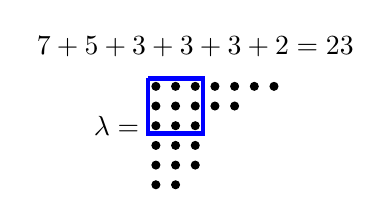
\begin{tikzpicture}
\draw (.5,.5) node {$7 + 5 + 3 + 3 + 3 + 2 = 23$};
\draw (-.5, -.5) node {$\lambda = $ };
\foreach \x in {0,...,6}
  \filldraw (\x*.25, 0) circle (.5mm);
\foreach \x in {0,...,4}
  \filldraw (\x*.25, -.25) circle (.5mm);
\foreach \x in {0,...,2}
  \filldraw (\x*.25, -.5) circle (.5mm);
\foreach \x in {0,...,2}
  \filldraw (\x*.25, -.75) circle (.5mm);
\foreach \x in {0,...,2}
  \filldraw (\x*.25, -1) circle (.5mm);
\foreach \x in {0,...,1}
  \filldraw (\x*.25, -1.25) circle (.5mm);
\draw[ultra thick, blue] (-.1,0.1) -- (-.1,-.6) -- (.6, -.6) -- (.6, .1) -- (-.1,.1);
\end{tikzpicture}
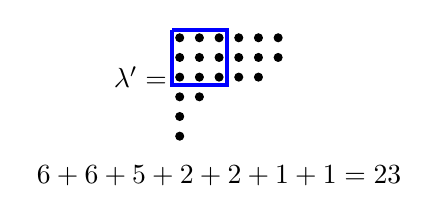
\begin{tikzpicture}
\draw (.5,-1.75) node {$6 + 6 + 5 + 2 + 2 + 1 + 1 = 23$};
\draw (-.5, -.5) node {$\lambda^\prime = $ };
\foreach \x in {0,...,5}
  \filldraw (\x*.25, 0) circle (.5mm);
\foreach \x in {0,...,5}
  \filldraw (\x*.25, -.25) circle (.5mm);
\foreach \x in {0,...,4}
  \filldraw (\x*.25, -.5) circle (.5mm);
\foreach \x in {0,...,1}
  \filldraw (\x*.25, -.75) circle (.5mm);
\filldraw (0, -1) circle (.5mm);
\filldraw (0, -1.25) circle (.5mm);
\draw[ultra thick, blue] (-.1,.1) -- (-.1,-.6) -- (.6, -.6) -- (.6, .1) -- (-.1,.1);
\end{tikzpicture}
\end{center}

There is a natural involution on the set of partitions of $n$, $\lambda\mapsto\lambda^\prime$.

The conjugate, $\lambda^\prime$ of $\lambda$ is the partition whose Ferrers' diagram is the transpose of that of $\lambda$.

{\color{red} \textbf{\underline{Exercise:}} Using the $(i_1, i_2, \cdots)$ descriptions of $\lambda$, express $\lambda^\prime$.}

\begin{definition}
The Durfee square of a Ferrers' diagram is the largest square which fits entirely inside the Ferrers' diagram.\\
A Durfee square has size $k$ if
\bea
\lambda_k & \ge & k\\
\lambda_{k+1} & < & k+1
\eea
\end{definition}

\underline{Observation:} $\lambda$ has all parts $\le k$ $\Longrightarrow$ $\lambda^\prime$ has at most $k$ parts.

\begin{corollary}
Fix $k$.
\bea
&&\text{generating function for partitions of $n$ into at most $k$ parts}\\
& = &\text{generating function for partitions of $n$ into parts of size at most $k$}\\
& = & \prod\limits_{j=1}^k \left(1 - x^j\right)^{-1}
\eea
\end{corollary}

\begin{corollary}
\bea
\prod\limits_{j=1}^\infty \left(1 - x^j\right)^{-1} & = & \sum\limits_{k = 0} ^\infty x^{k^2} \prod\limits_{j=1}^k \left(1 - x^j\right)^{-2}
\eea
\end{corollary}
\begin{center}
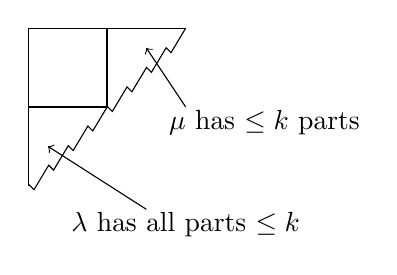
\begin{tikzpicture}
\draw (0,0) -- (1,0) -- (1,1) -- (0,1) -- (0,0);
\draw (1,1) -- (2,1);
\draw (0,0) -- (0,-1);
\draw[decorate, decoration=saw] (2,1) -- (0,-1);
\draw[->] (2,0) -- (1.5, .75);
\draw (3,-.2) node {$\mu$ has $\le k$ parts};
\draw[->] (1.5,-1.3) -- (.25, -.5);
\draw (2,-1.5) node {$\lambda$ has all parts $\le k$};
\end{tikzpicture}
\end{center}
\end{document}